
\setcounter{section}{0}
\setcounter{figure}{0}
\graphicspath{{./figs/}{./figs/item-rajiv/}}

\NewsTitle{Cyber-Physical-Social Clouds: Future Insights}
\NewsAuthor{Rajiv Ranjan$^1$, Prem Prakash Jayaraman$^2$, Ellis Solaiman$^1$, and Dimitrios Georgakopulos$^2$\\
$^1$School of Computing Science, Newcastle University, United Kingdom \\
$^2$School of Computer Science and Information Technology, RMIT University, Australia}


Cyber-physical systems (CPS) are a vast interlinked network of things/devices, computing resources, applications/services and humans, that use a range of sensors, actuators and communication topologies,
to link the computations systems (platforms) with the physical world.
CPS drives the vision of a ``smart interconnected cyber social world'' where the physical social world is monitored by sensors in real time,
and the services in the cyber world use the data to directly influence the decision making in the physical world.

The Internet of Things (IoT) and cloud computing are integral parts of the cyber-physical- ecosystem \cite{ref4}.
While the IoT is seen as the means for connecting disparate sensing and actuation devices (via the Internet) with applications and services,
cloud computing offers computation and storage capabilities required by those data processing applications and services.
Aided by the low cost and availability of wired and wireless networking technologies as well as cheap sensors and actuator devices,
the IoT will transform the Internet into a fully integrated smart environment where large amounts of generated data can be shared across diverse applications and platforms.
The social impact of connecting clouds and IoTs to form such smart environments will be a revolution that promises to change people's lives across a variety of domains including;
smart homes and smart cities with smart management systems for traffic management and accident prevention,
intelligent advanced warning systems to help communities with prediction and preparation for environmental conditions such as storms and floods,
and smart healthcare monitoring delivering immediate automated on demand and real time data on the wellbeing of patients. 

CPS takes advantage of cloud's pay-as-you go model to support various applications such as emergency health care, evacuation and rescue systems, disaster-management applications, and personal fitness systems.
The NIST definition \cite{ref1} of cyber-physical cloud computing is
``a system environment that can rapidly build, modify and provision cyber-physical systems composed of a set of cloud computing based sensor, processing, control, and data services''.
Based on this definition, we define the cyber-physical-social clouds as ``an ecosystem of tools, frameworks and systems that can facilitate rapid development, deployment and management of cyber-physical applications composed of Things (sensors and actuators), Clouds (processing, control, data services and applications) and Humans (Social bounded by a closed loop data flow relationship''. 

Figure \ref{fig:fig1} provides an overview of the Cyber-Physical-Social Clouds (CPSC) using an onion model to describe the expanding and extending relationship between various layers.
As depicted in the figure, the Physical space is composed of embedded systems that could include a range of sensing and actuation devices (e.g.~wireless sensor networks),
things (e.g.~fitbit), smart phone and smart vehicles (e.g.~google car).
They are interwoven with various ubiquitous communication capabilities allowing them to be networked (e.g.~Internet).
The cyber cloud hosts applications, services supported by big data processing components (such as Apache spark, Hadoop etc.), in order to process, analyse and compute actionable outcomes from the sensed data.
The actionable responses are propagated back into the physical world via actuators.
The cyber-physical ecosystem also encompasses a human aspect wherein humans provide data, act on analysed data and make informed decisions. 

The components of CPSC namely the IoT and cloud are very distinct and complimentary.
While IoT provides localization, therefore enabling low latency and context awareness, the cloud provides global centralization.
Further, Clouds offer virtually unlimited, scalable access to resources (computing, storage) while IoT is generally conceived as a resource constrained environment.
Finally, IoT bring with it the sheer scale (estimated to be 50 billion devices by 2020 \cite{ref2}) and complexity.

\begin{figure}[htbp]
	\centering
    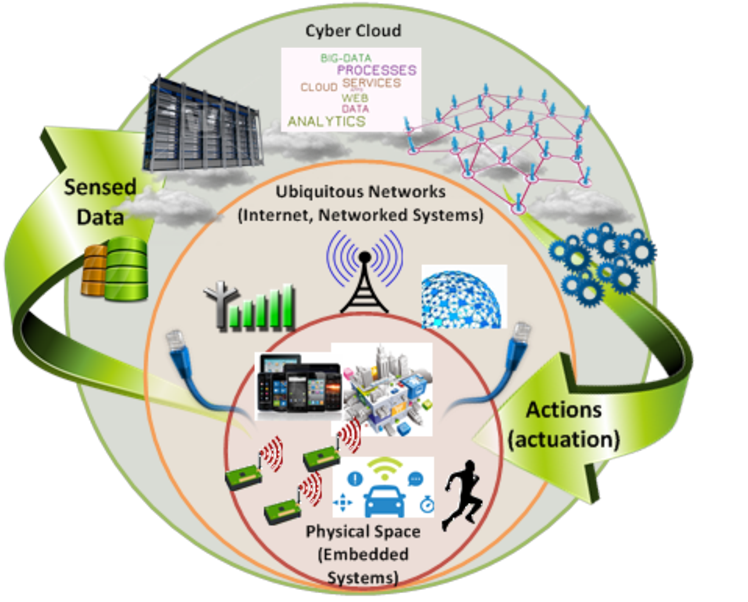
\includegraphics[width=0.72\linewidth]{fig1}
	\caption{Cyber-Physical Clouds}
	\label{fig:fig1}
\end{figure}

Rapid advances in IoT (e.g.~mobile computing, man-machine, machine-machine communications, and smart phone networks) will cause a paradigm shift in the design of CPSC applications and operations,
by bringing improvements not only to the quality of service (QoS) but also to quality of experience (QoE), cost efficiency, reliability, security, and energy efficiency.
Moreover, resources in data centers and cloud infrastructures have to be efficiently managed and scheduled to optimize reliability and scalability of CPSC under various constraints of QoS and QoE.
Besides, CPSCs are expected to deal with data directly coming from trans-domain applications (e.g.~traffic accident detection in smart transportation, energy management in smart grid, health monitoring and evaluation),
which could be in various forms such as GPS coordinates, flood level, temperature, rainfall rate, vehicle speed, electricity consumption, etc.
How to coordinate various applications of heterogeneous systems and facilitate a deeper integration, interaction and personalization of the physical, cyber, and social domains is an important challenge.
In order to build the next generation CPSC applications and services, it is essential to address the challenges introduced by IoT and Clouds while leveraging on their advantages.


\section*{Challenges:}

In this newsletter, we highlight some of the key challenges that need to be addressed in order to develop scalable, reliable and cost-efficient CPSC applications and services. These include:

\textbf{Real-time data processing, and actuation}:
IoT is tightly bound by its real-time data processing and its subsequent analysis that can help with driving decisions making processes.
Hence, CPSC applications require the development of models to reduce latency and inefficient communication between Clouds and IoT in order to achieve real-time data processing and actuation needs. 

\textbf{Multi-tenancy Clouds}:
IoT is a distributed system that produces enormous amounts of data.
In fact, IoT is considered a major source of Big-data.
Hence, there is a need to support storage and processing of un-structured and semi-structured big data coming from distributed sources to provide real-time/near real-time services.
This will require multi tenancy cloud models to meet the scalability and real-time needs of CPSC applications.

\textbf{Dependable QoS management}:
CPSCs bring unique challenges in the form of IoT that is very different to traditional cloud-based applications.
For example, CPSC system performance is based not only on the Clouds but also the IoT devices.
Hence, careful consideration and prediction of QoS and corresponding SLAs is key for CPSC applications.
These QoS metrics could include performance targets/constraints of CPSC applications, distributed processing and storage of the massive data as well as run-time migration of cloud servers (VMs).

\textbf{Discovery and Service Composition (Clouds and IoT)}:
Discovery is a mechanism that will enable users and application likewise to find and access Cloud services and corresponding IoT data without the need to know the actual source of the data, sensor description, or location.
An intrinsic requirement of CPSC applications is to manage heterogeneity at various level such as different types of sensors, data and cloud services.
Currently the standards that govern the development of these components are at their infancy.
Even with appropriate standards, given the growth rate of IoT, it is expected that we will soon face the challenge of integrating a multitude of devices and data stemming from IoT.
Hence, there needs to be mechanisms that allows the discovery of these IoT devices and the corresponding services (e.g.~storage service) that fit the requirement of the CPSC applications.

\textbf{CPS identity management}:
In the CPSCs, a service provider could potentially receive data from hundreds of data sources.
The provider needs to be able to determine to which end user the data belongs to \cite{ref3}.
In addition to data and data source identification \cite{ref3}, we need to be able to both specify and identify to which user/s the `thing/s' belongs to,
thus determining the context (e.g.~relating to which person) in which a particular sensor or actuator is operating.
Sensors could be shared and generate data that is relevant to a number of different users.
For example a proximity sensor in a hospital should identify when particular staff or patients are near it.
When the ``things'' are actuators, it becomes particularly important that the right actions are triggered for the right actors.
Also, conflicts might arise.
In a home IoT scenario, different members of a family may have different temperature preferences, so policies over thermostat control could conflict.
In such cases and others, policy conflict detection and resolution mechanisms maybe of utmost importance. 

\textbf{Virtualised Cloud IoT}:
CPSC systems provide a unified view of the physical world to the cyber user and vice-versa.
Hence, it is essential to maintain a virtual environment that represents the physical world monitored by the IoT devices.
This will require the development of various domain ontologies and corresponding reasoning techniques that can best describe the current physical world consistently in order to facilitate discovery and service composition.

\textbf{Emerging CPSC business models}:
CPSC is still in its infancy and so is challenged by the development of relevant and appropriate business models.
E.g.~the classical cloud model may no longer be applicable as CPSC is not only about the computer resources, it encompasses the IoT and the social aspects (humans).
Hence, business models need to be developed that takes into consideration all the 3 factors of CPSC namely, IoT, Clouds and Humans.

\textbf{Platforms for CPSC development and deployment}:
The development of CPSC systems is not a trivial task and requires careful consideration of various aspects including the construction and deployment of IoT infrastructure and cloud infrastructure,
while giving due diligence to the social aspect.
The question here is what could be the essential features of a cloud-based frameworks for CPSCs in order to support the right level of development techniques and methodologies?


\bibliographystyle{plain}
\begin{thebibliography}{10}

\bibitem{ref1}
Eric D.~Simmon, Kyoung-sook Kim, Eswaran Subrahmanian, Ryong Lee, Frederic J.~de Vaulx, Yohei Murakami, Koji Zettsu, and Ram D.~Sriram,
\newblock{``A Vision of Cyber Physical Cloud Computing for Smart Networked Systems''},
\newblock{\em NIST Interagency/Internal Report (NISTIR) -- 7951}, August 26, 2013.

\bibitem{ref2}
Cisco,
\newblock{``Internet Of Things Will Deliver \$1.9 Trillion Boost To Supply Chain And Logistics Operations''},
April 15, 2015, \url{http://newsroom.cisco.com/press-release-content?articleId=1621819}.

\bibitem{ref3}
P. N. Mahalle, B. Anggorojati, N. R. Prasad, and R. Prasad,
\newblock{``Identity Authentication and Capability Based Access Control (IACAC) for the Internet of Things''},
\newblock{\em Journal of Cyber Security and Mobility}, vol.~1, no.~4, pp.~309--348, 2013.

\bibitem{ref4}
L.~Wang and R.~Ranjan,
\newblock{``Processing Distributed Internet of Things Data in Clouds''},
\newblock{\em IEEE Cloud Computing}, Vol.~2, No.~1, Feb 2015, BlueSkies Column, IEEE Computer Society. 

\end{thebibliography}

